\documentclass{article}
\usepackage[]{changepage}
\usepackage[]{realtristan}
\title{Physics Light and Waves Summary}
\author{Tristan Simpson}
\begin{document}
\maketitle
\tableofcontents

\vspace{1\textwidth}
\section{Bubbles and Films}
\subsection{Fixed and Free Ends}
When a wave hits a fixed end (fast medium to slow medium), the resulting wave (phase) is reflected. When a wave hits a free end (slow medium to fast medium), the resulting wave is reflected.\\
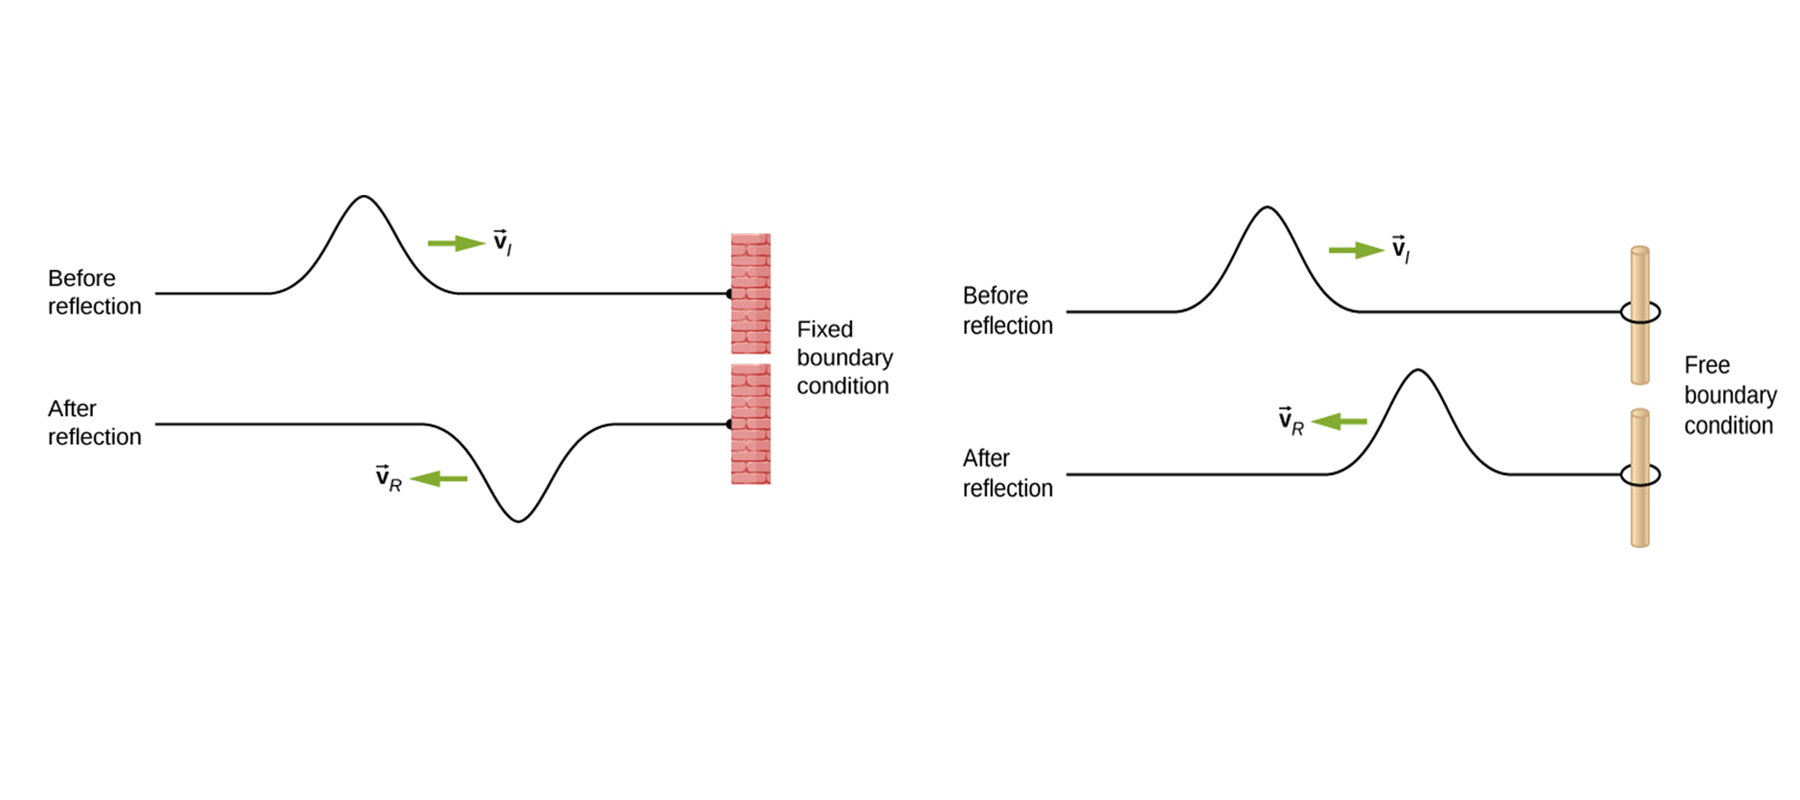
\includegraphics[scale=3]{images/fixed_free_ends} \\
\vspace{-2cm}
\subsection{Mediums}
So what is a medium? A medium is the material that the wave is travelling through. A great example of mediums, directly correlating to this unit, are air and water. Air is a fast medium, and water is a slow medium.\\

\subsection{Bubbles as a Film}
As the light wave travels from the air medium ($n_{air}$) to the soap medium ($n_{soap}$), the phase is reflected back to the persons eye and the original wave is inverted into the bubble. The original wave is then reflected back to the persons eye after bouncing around inside the bubble. The person now see's two reflected lights. Depending on the thickness of the film ($t$), the reflected light ($R$) and the original light ($O$) will either constructively or deconstructively interfere.\\\\
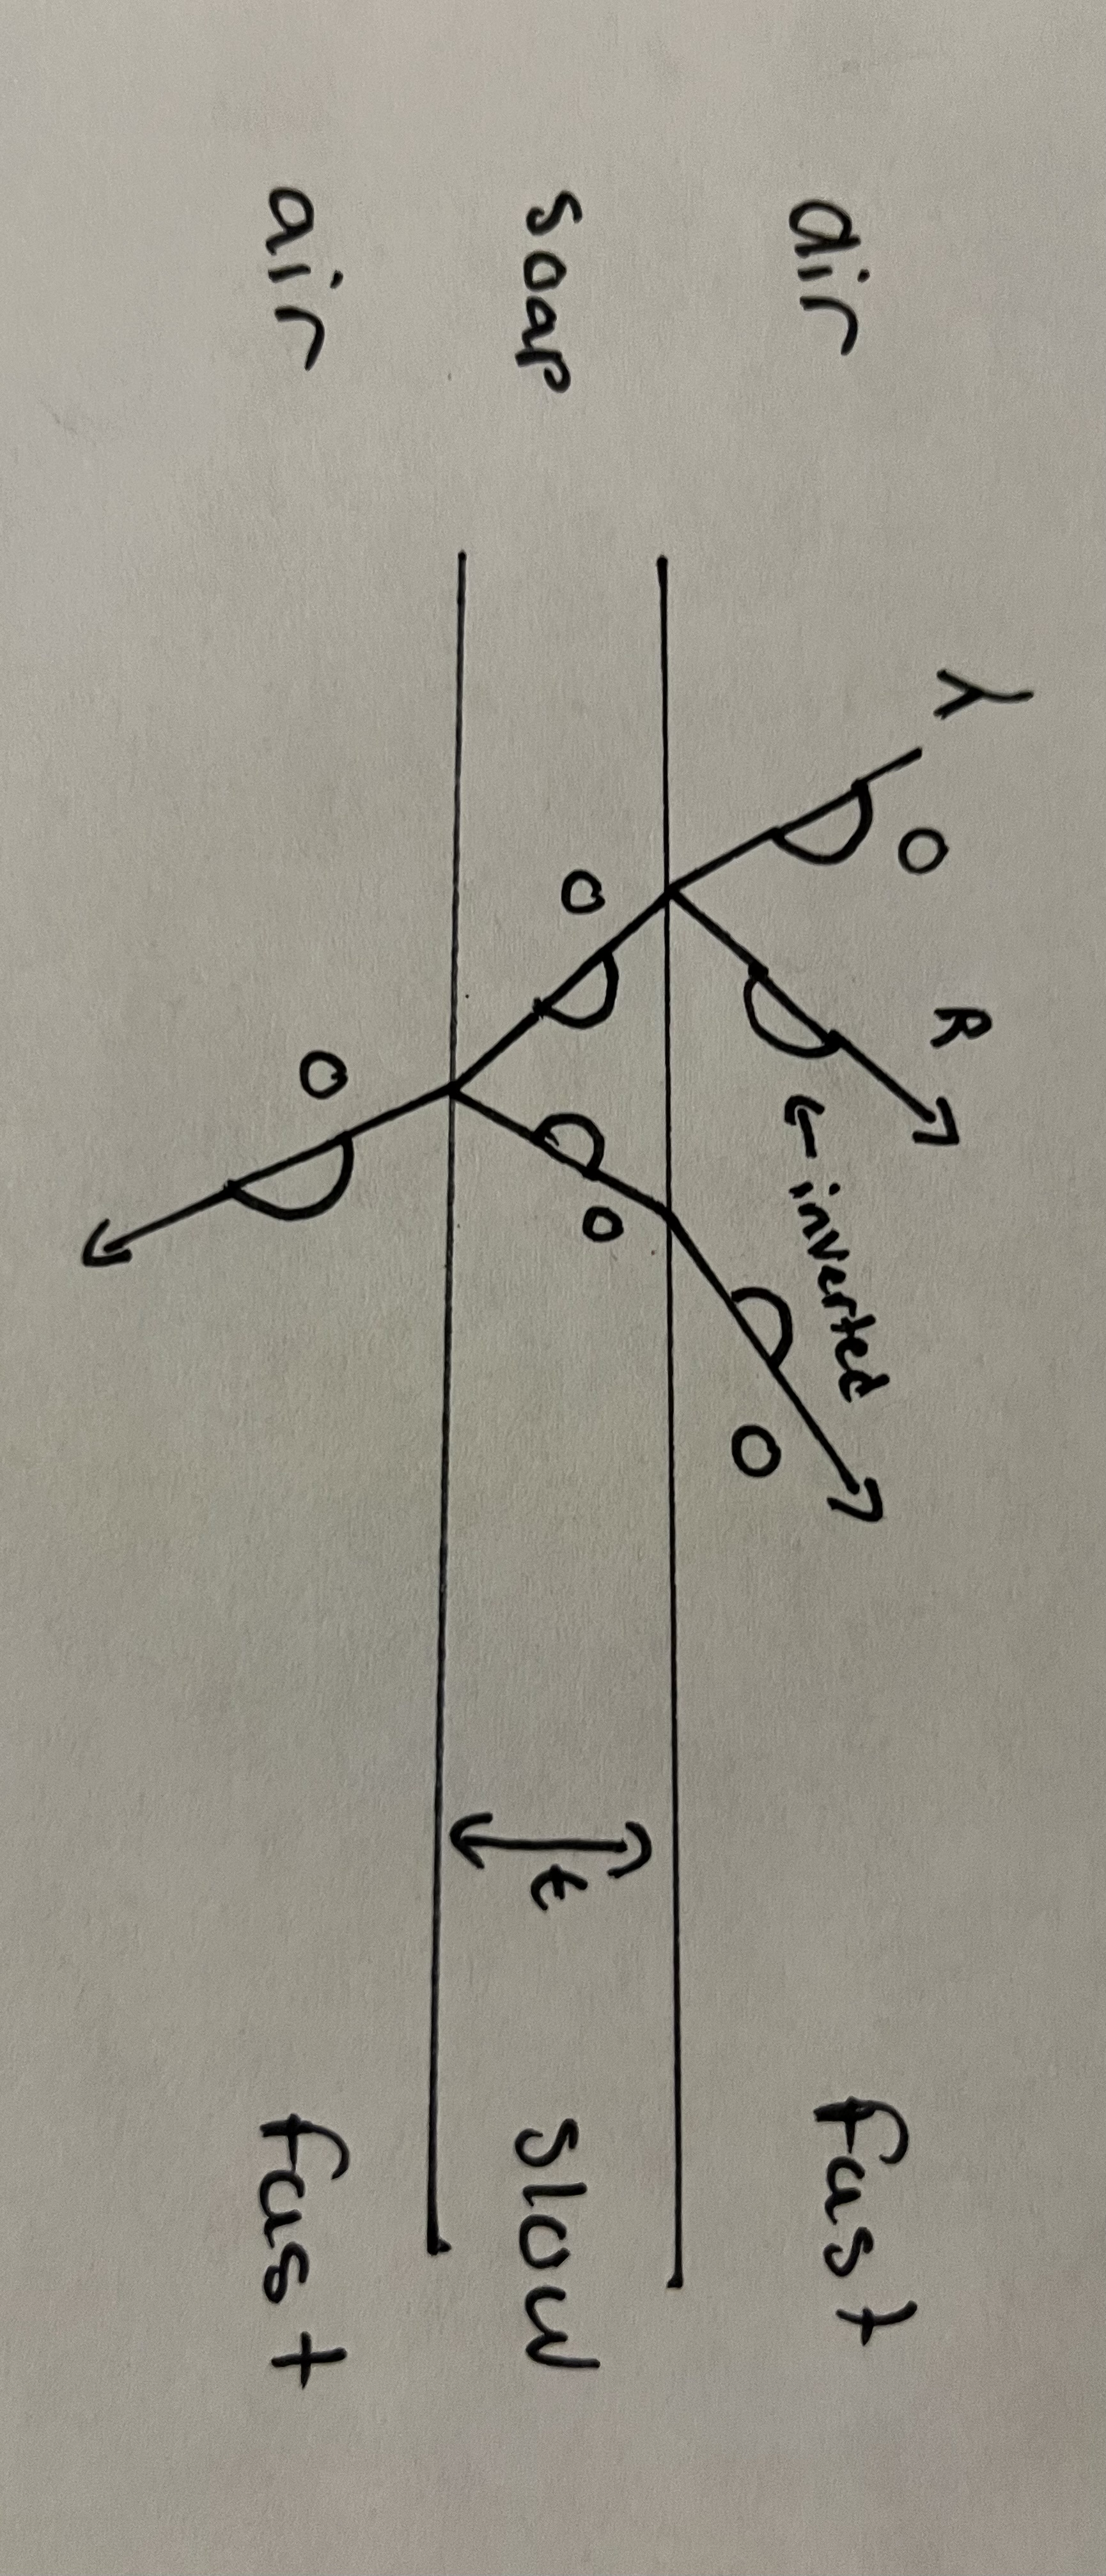
\includegraphics[scale=0.05, angle=90, origin=c]{images/bubble_lens}

\subsection{Reflected Film Light}
If a second wave is out of sync with the original wave, the two waves will either deconstructively or constructively interfere by the time they reach a screen (eye, screen, table, etc.) which will result in seeing either a bright or dark spot.\\\\
If the thickness of a film is very, very thin, (practically zero), then the waves will be in sync because the distance is negligible. \\\\
If the thickness of a film is thicker, then the waves, depending on the thickness of the film, will potentially be out of sync. \\\\
This is because $Wave_2$ has to travel farther than $Wave_1$ post it's reflection on the bottom of the film, to reach the screen.\\\\
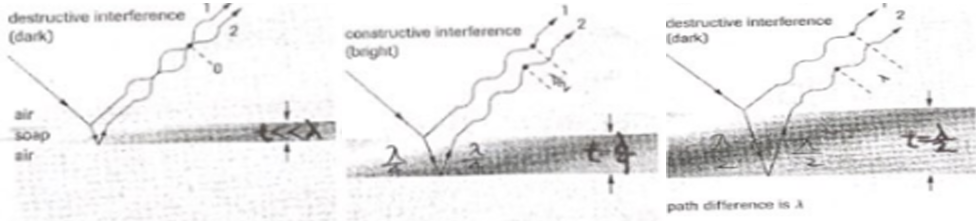
\includegraphics[scale=0.5]{images/reflected_films} \\\\
\noindent \textbf{Reflection Constructive Interference (Bright):} $\frac{\lambda}{4}$, $\frac{3\lambda}{4}$, $\frac{\lambda}{4}$ \\\\
\textbf{Reflection Deconstructive Interference (Dark):} $0$, $\frac{\lambda}{2}$, $\lambda$, $\frac{3\lambda}{2}$ \\\\

\subsection{Transmitted Film Light}
The transmitted film light constructive and deconstructive interference equations are the exact opposite of the reflected film light constructive and deconstructive interference equations.\\\\
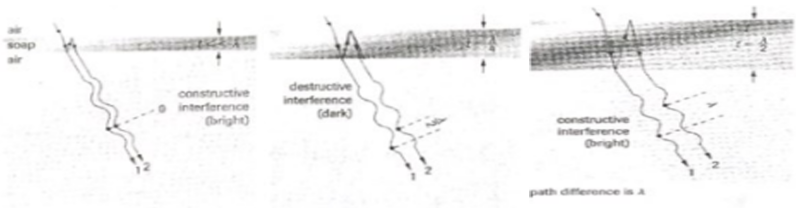
\includegraphics[scale=0.5]{images/transmitted_films} \\\\
\noindent \textbf{Reflection Constructive Interference (Bright):} $0$, $\frac{\lambda}{2}$, $\lambda$, $\frac{3\lambda}{2}$ \\\\
\textbf{Reflection Deconstructive Interference (Dark):} $\frac{\lambda}{4}$, $\frac{3\lambda}{4}$, $\frac{\lambda}{4}$ \\\\

\section{Single and Double Slits}
\subsection{Theory}
\textbf{If Young's Double Slit Experiment were to be submerged in water, how would the fringe pattern change?}\\\\
The length of a wave ($\lambda$) is strongly dependant on it's medium. If the experiment was to be submerged in water (a slower medium than air), then the wavelength of the light would decrease and the fringe pattern would become closer together.\\\\

\noindent\textbf{2. For diffraction by a single slit, what is the effect of increasing (a) the slit width, and (b) the wavelength?}\\\\
(a) Increasing the slit width ($d$) would decrease the width of the central maxima. This is proven by the equation: $\Delta y = \left(\frac{(\lambda)(L)}{d}\right)$\\\\
(b) Increasing the wavelength ($\lambda$) would increase the sie of the central maxima. This is proven by the equation: $\Delta y = \left(\frac{(\lambda)(L)}{d}\right)$\\\\

\subsection{Wavelets}
Christiaan Huygens use of "wavelets" describes the interference pattern created by a single slit. Wavelets are a wave split into multiple miniatures lines and depending on the $\theta$ of these lines, the screen (or eye, etc.) will experience either constructive or deconstructive interference.\\

\noindent\textbf{Deconstructive Interference}\\
If the path difference from one side of the slit to the other is a multiple of $\lambda$ (eg. $2\lambda$, $3\lambda$, ...), then there will be deconstructive interference.
\begin{align*}
    y_m = \left(\frac{m\lambda L}{w}\right)\;\; where\;\;(m\;=\;\pm 1,\;\pm 2,\;\pm 3,\;\pm 4,\;...)
\end{align*}\leavevmode\\\\\\\\\\

\noindent\textbf{Constructive Interference}\\
If the path difference from one side of the slit is off by half a wavelength (eg. $\lambda + \frac{1}{2}$), then there will be constructive interference.
\begin{align*}
    y_m = \left(\frac{(m + \frac{1}{2})\lambda L}{w}\right)\;\; where\;\;(m\;=\;\pm 1,\;\pm 2,\;\pm 3,\;\pm 4,\;...)
\end{align*}\leavevmode
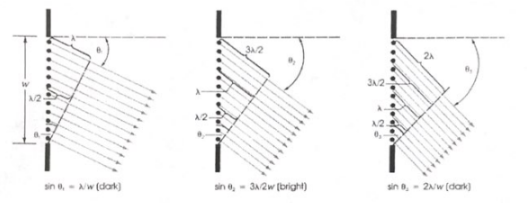
\includegraphics[scale=0.8]{images/wavelets} \\

\subsection{Patterns}
The patterns below are the result of a single slit and a double slit. The intensity's of the fringes are also shown. The highest points of the intensities are called the maximas, and the lowest points of the intensities are called the minimas.\\\\
\begin{minipage}{0.5\textwidth}
    \textbf{Double Slit Pattern $\Delta y = \frac{(\lambda)(d)}{L}$} \\
    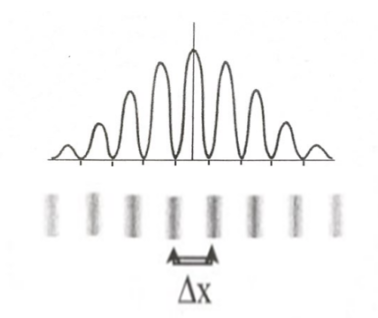
\includegraphics[scale=0.5]{images/double_slit_pattern} \\
\end{minipage}
\begin{minipage}{0.5\textwidth}
    \vspace{10pt}
    \textbf{Single Slit Pattern $\Delta x = \frac{(\lambda)(d)}{L}$} \\
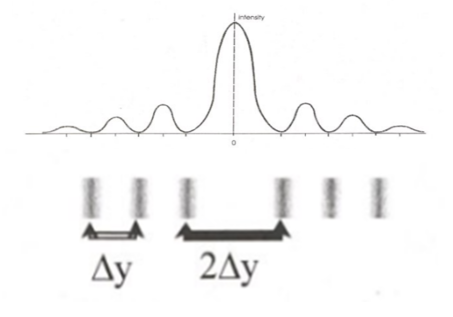
\includegraphics[scale=0.5]{images/single_slit_pattern} \\\\
\end{minipage}

\subsection{Diffraction}
When a light wave passes through a narrow slit, the wave diffracts. This diffraction is only noticeable by the human eye when $\frac{\lambda}{d} \geq 1$ \\\\
The interference pattern created by the single slit is from wavelets. The interference pattern created by the double slit is from the waves overlapping eachother, causing constructive and deconstructive interference. \\\\
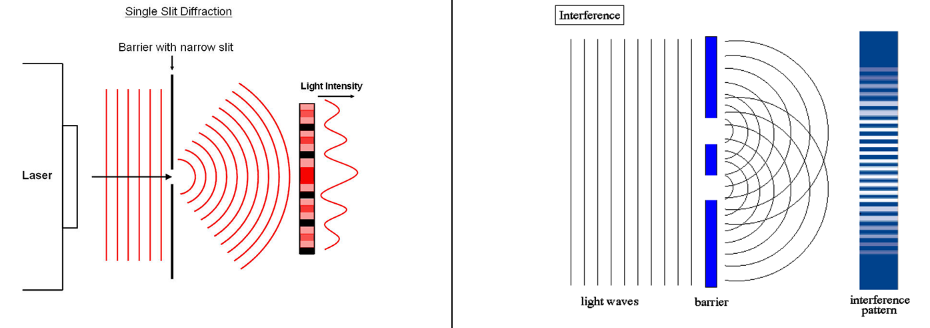
\includegraphics[scale=0.4]{images/slit_diffraction} \\

\section{Diffraction Gratings}
Young's Double Slit apparatus inspired the diffraction grating. The diffraction grating is a series of NUMEROUS slits (not just the two from young's "double" slit) that are very close together.\\
\begin{itemize}
    \item Diffraction Gratings gave physisists a much more accurate measurement of the wavelength of the light source.
    \item The name "Diffraction Grating" comes from the fact that the light waves diffract when as they travel through the tiny slits cut into the apparatus.
    \item Holding a diffraction grating to a source of \textbf{white light} easily splits the light into a rainbow of colors.
    \item The patterns created by a diffraction grating still consist of maximas (bright regions / high intensities) and minimas (dark regions / low intensities) except the maximas become very narrow and well defined.
    \item Using monochromatic light you can see very distinct bright and dark fringes.
\end{itemize}\leavevmode\\
\noindent\textbf{Image of Diffraction Grating:}
The light doesn't travel through the black lines. The light travels through the white lines. These lines act as mini slits.\\\\
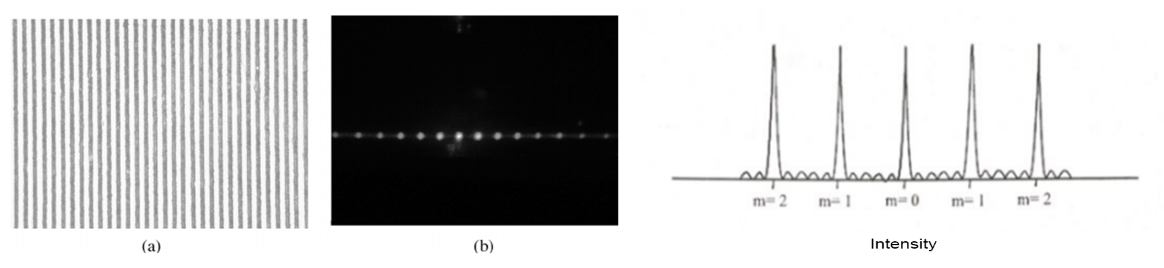
\includegraphics[scale=0.4]{images/diffraction_grating} \\

\section{Polarization}
Polarization is the splitting of waves into their components.\\\\
Light waves have both vertical and horizontal components. The horizontal component is called the "electric field oscillation" and the vertical component is called the "magnetic field oscillation".\\
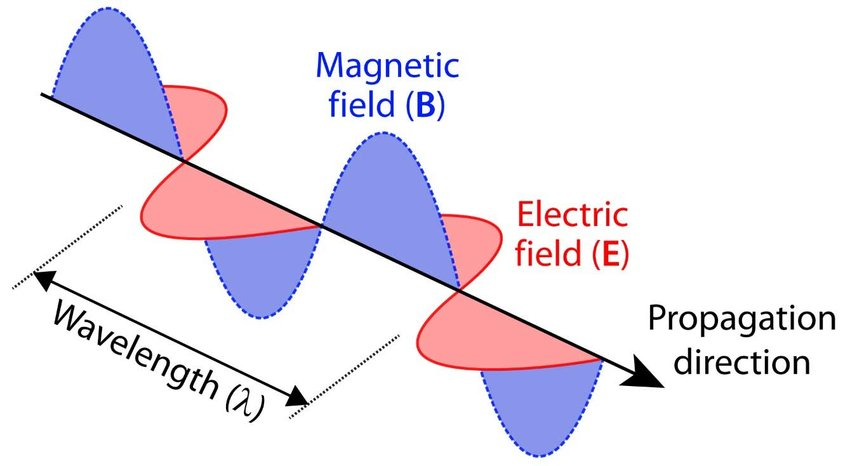
\includegraphics[scale=0.25]{images/wave_components} \\

\noindent As a light wave travels through a polarized lense, either the magnetic field component or the electric field component is eliminated, leaving only one of the two components.\\\\
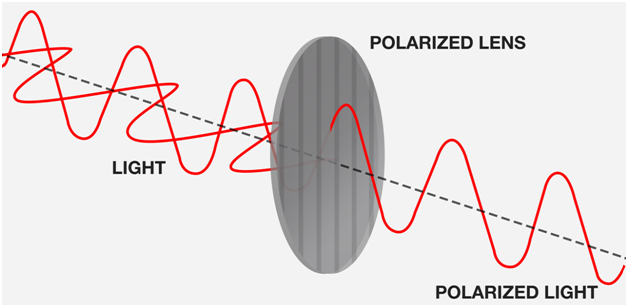
\includegraphics[scale=0.33]{images/polarized_lens} \\

\noindent As an example, if you put together vertically polarized lense and a horizontally polarized lense in their corresponding directions, the light will not be able to move through the lense. \\\\
If you rotate one of the lenses 90 degrees, the light will be able to pass through the lense because the polarized component is now the same as the other. \\


% Double Slit Equation 1
\section{Double Slit Equations (1)}
Monochromatic light falls on two slits 0.024 mm apart. The fringes on a screen 3.00 m away are 6.7 cm apart. What is the wavelength of light?
\subsection*{Givens}
\begin{itemize}
    \item $d = 2.4 \times 20^{-5}\;m$
    \item $L = 3.00\;m $
    \item $\Delta x = 6.7 \times 10^{-2}\;m$
\end{itemize}\leavevmode
\subsection*{Solve}
To solve for the wavelength of the light, we can use the equation $\lambda = \left(\frac{(\Delta x)(d)}{L}\right)$\\ Our result should be in meters, but if converted, the result should be in nanometers.\\
\begin{align*}
     & \lambda = \left(\frac{(\Delta x)(d)}{L}\right)      = \left(\frac{(6.7 \times 10^{-2})(2.4 \times 10^{-5})}{3.00}\right) \approx 5.20 \times 10^{-7}\;m
\end{align*}\leavevmode\\

% Double Slit Equation 2
\section{Double Slit Equations (2)}
A parallel beam of 700 nm light falls on two small slits $6.0 \times 10^{-2}$ mm apart. How wide would a pattern of eight bright fringes be on a screen 3.0 m away?
\subsection*{Givens}
\begin{itemize}
    \item $d = 6.0 \times 10^{-5}\;m$
    \item $\lambda = 7.0 \times 10^{-7}\;m$
    \item $L = 3.0\;m$
\end{itemize}\leavevmode
\subsection*{Solve}
To solve for the width of the pattern of eight bright fringes, we must first solve for the distance between two ($\Delta x$). After solving for $\Delta x$ we can multiply it's value by eight to get the final distance.\\
\begin{align*}
     & \Delta x = \frac{(\lambda)(L)}{d} = \left(\frac{(7.0 \times 10^{-7})(3.0)}{6.0 \times 10^{-5}}\right) \approx 3.5 \times 10^{-2}\;m \\\\
     & \therefore\;\;(8)\Delta x = (8)(3.5 \times 10^{-2}) \approx 2.8 \times 10^{-1}
\end{align*}\leavevmode\\

% Single Slit Equations
\section{Single Slit Equations (1)}
How wide is the central diffraction peak on a screen 2.50 m behind a 0.0212 mm wide slit illuminated by 550 nm light?
\subsection*{Givens}
\begin{itemize}
    \item $L = 2.50\;m$
    \item $d = 2.12 \times 10^{-5}\;m$
    \item $\lambda = 5.5 \times 10^{-7}\;m$
\end{itemize}\leavevmode
\subsection*{Solve}
To solve for the width of the central maxima we use a formula very similar to the one used in the double slit calculations: $\Delta y = \left(\frac{(\lambda)(L)}{d}\right)$ Where $\Delta y$ is the width of the central maxima.\\
\begin{align*}
     & \therefore\;\;\Delta y = \left(\frac{(\lambda)(L)}{d}\right) = \left(\frac{(5.5 \times 10^{-7})(2.50)}{2.12 \times 10^{-5}}\right) \approx 6.5 \times 10^{-2}\;m
\end{align*}\leavevmode\\

% Single Slit Equation 2
\section{Single Slit Equations (2)}
How wide is a slit if it diffracts 690 nm light so that its central peak is 3.0 cm wide on a screen 2.80 m away?
\subsection*{Givens}
\begin{itemize}
    \item $L = 2.80\;m$
    \item $ \Delta y = 3.0 \times 10^{-2}\;m$
    \item $\lambda = 6.9 \times 10^{-7}\;m$
\end{itemize}\leavevmode
\subsection*{Solve}
To solve for the width of the single slit we can rearrange the formula from the solve above. $\Delta y = \left(\frac{(\lambda)(L)}{d}\right)$ $\to$ $d = \left(\frac{(\lambda)(L)}{\Delta y}\right)$.\\
\begin{align*}
     & \therefore\;\;d = \left(\frac{(\lambda)(L)}{\Delta y}\right) = \left(\frac{(6.9 \times 10^{-7})(2.80)}{3.0 \times 10^{-2}}\right) \approx 6.44 \times 10^{-5}\;m
\end{align*}\leavevmode\\

\end{document}